\documentclass[12pt, man, natbib, marker]{apa6} % man: manuscript
%\usepackage{natbib}
\usepackage{times}
\usepackage[USenglish]{babel}
\usepackage{rotating}
%\usepackage{color}
\usepackage{url}

\usepackage{booktabs}
\usepackage{longtable}
\usepackage{array}
\usepackage{multirow}
\usepackage{wrapfig}
\usepackage{float}
\usepackage{colortbl}
\usepackage{pdflscape}
\usepackage{tabu}
\usepackage{threeparttable}
\usepackage{threeparttablex}
\usepackage[normalem]{ulem}
\usepackage{makecell}
\usepackage{xcolor}

\usepackage{makecell}

\urldef\repository\url{https://github.com/julianbarg/oil_industry}

\title{Valuing Peace and Quiet: the Effect of Expansion Mode on Learning toward Subordinate Goals}
\shorttitle{Valuing Peace and Quiet}
\author{Julian Barg\\barg.julian@gmail.com}
\affiliation{Ivey Business School}
\setcitestyle{authoryear, open={(},close={)},citesep={,},aysep={}}
%\bibliographystyle{plainnat}

% \abstract{The topic of temporality has been analyzed from multiple different angles. In this paper, we develop a working definition of corporate pace, a new concept in this field. Most previous studies of temporality focus on the time frame of decisions, or perception of time. Corporate pace on the other hand describes how frequently major changes are being implemented. When frequent swift changes take place, the content of individual decisions matters less. The fast pace becomes an important characteristic that affects the development of the firm. We argue that the fast pace can cause breakdowns of important routines, and thus define a new starting point for research on occurances of accidents and environmental impacts.}


\begin{document}
	
\maketitle

\section{Introduction}
We observe organizational learning in the context of pipeline operators. The task and large parts of the environment (technology and immediate surrounding) of pipeline operators compared to other industries are very stable. The industry is yet to be disrupted by renewable energy in a major way. The only major source of disruptions are internal adjustments to strategy, such as the construction of a new pipeline, or the acquisition of a competitor. In the 2010s constructed almost a hundred thousand miles of new pipelines (as of 2018), in response to the fracking boom of the US oil and gas sector. In 2018, 406 pipeline incidents occurred, 151 of which were classified by the Federal Energy Regulatory Commission (FERC) as "significant". We track how companies handle their pipeline system extensions, and how the mode of development (i.e, stable or with many strategic adjustments) affects their incident rate.

The organizational goal of a pipeline operator (or extraction company with pipeline assets) is not identical with that of its suborganizations: the parent organization may respond to the business case for new pipelines, or pipeline acquisitions, for instance when new oil fields are discovered. The right portfolio of pipelines at the right time allows the organization to maximize profits. The department that is in charge of pipeline safety does not contribute to revenue generation - it is "sunk cost" in the best case, and a drain on profits when incidents occur. In the worst case, a streak of bad enough oil spills can threaten the existence of a smaller operator, such as HVI Cat Canyon: this small pipeline operator went bankrupt in 2019 after a number of pipeline leaks (in California, where laws are relatively stringent) led to a series of lawsuits; the organization could not afford to pay the fines \citep{WSJ2019}. Learning in this context occurs on separate organizational levels. \citet{Cyert1992} explains that an organization's \textit{aspiration level} drives activity at the organizational level; for instance, a company in the oil industry perceiving a shortfall in performance relative to its reference group might acquire new oil fields or construct a new pipeline to reach a new market. Pipeline safety at this level is a \textit{hygiene factor}: a certain level of performance is required for survival, but beyond that level, an improved pipeline safety does not make a large difference for competing in the market. Most importantly, pipeline safety is left censored: once you have achieved perfect safety, additional effort is wasted; further, the cost of making additional progress beyond a certain point by controlling for all eventualities might increase exponentially; hence, the organization may have an economic interest of not over-optimizing performance in this are (since once perfect safety is achieved, the additional effort does not yield any return).

This focus (on overall revenue or profit growth) constitutes a significant difference from the goals of the business unit that operates the pipelines. An oil spill can threaten careers in and the success of this department, while the department and its members cannot distinguish themselves through outstanding performance and achievements. The best case scenario for the pipeline safety is not to stand out excellent performance in an initiative, but to stand out through from the lack of anything happening. Hence, this department's interest is to prevent incidents. The safety track record is related to the overall organizational goal (of survival, or attaining the aspiration level), but it is not identical with the overarching organizational goal - pipeline safety is a subordinate goal. When given the opportunity, a department can learn and make strides toward its subordinate goal: the learning curve applies for a goal when an organization can gain experience by carrying out the same task repeatedly \citep{Argote2013_1}. When the organization is disrupted however (for instance because the parent organization implements changes), the learning process may be interrupted, and existing knowledge can become irrelevant or depreciate \citep[pp. 62 ff.]{Argote2013_3}. The learning curve is "reset".

In the context of pipeline operations, we test the relationship between parent organization activities and the suborganization's learning toward their subordinate organizational goal. The resetting of the learning process suggests that in time periods of stability, when the parent organization's activities are relatively constant, the department in charge of pipeline safety can engage in learning toward its subordinate organizational goal. When a big change occurs as the result of the parent organization's activities (e.g., the commissioning of a new pipeline), the department learning curve is disrupted and the department experiences a set back on the learning curve (now learning toward the operating safety of the overall, new system), thus, activities are less optimized and errors are more likely.

To measure disturbances from the overall organization, we turn to expansions of the pipeline network. The context of pipeline operators provides a unique research opportunity: US regulations mandate that organizations provide data on their pipeline network annually, and for FERC to provide this data to the public. Thus, we know the exact scope of pipeline operators across time. For our purpose this dataset is more suitable than accounting data, which can be less comparable across years or organizations due to different ways of depreciating assets, boosting revenue, etc. We measure how even an operator's rate of change is across years - we expect time periods of relatively steady rate of change to allow for suborganizations to learn and drive down incident rates. Incident counts are also provided by FERC, to which companies are obliged to report oil spills that either (1) led to a loss of 19l of liquid or more, (2) resulted in a personal injury, or (3) cause a property damage of \$50,000 or more.

{Organizational Learning, Forgetting, and Disruptions}
Strategic approaches to development vary substantially, even between seemingly similar companies. \citet{Morales-Raya2015} describes the different approaches that the Coca-Cola Company and PepsiCo have taken over the years: Coca Cola has taken more initiatives to capture new markets and generally "moved fast" where it saw a business opportunity, but often with sloppy execution. Pepsi has relied less on radical, ambitious new projects, yet, over time managed to achieve a higher market capitalization. The strategic approach that the top management of a company takes determines how well an organization can learn from new experiences, and build on existing knowledge. In the quickly moving environment of Coca-Cola, high-profile mistakes occurred at a higher rate. The three determining factors the impact of top level action on organization-wide learning are \textit{knowledge depreciation}, \textit{disruptions} and opportunities for learning, e.g., \textit{vicarious learning}.

\subsection{Knowledge Depreciation/Organizational Forgetting}

The learning curve (in its many different iterations) famously showcases how an organization over time drives down the unit cost of goods \citep{Wright1936} or services, and that the organization can over time improve other performance metrics also \citep[p. 1]{Argote2013_1}. For some time, an implicit assumption underlying this research stream has been that organizational knowledge is cumulative, that it "persists indefinitely through time" \citep[p. 57]{Argote2013_3}. If that was the case, the mode of extension should not be a concern for pipeline operators (or companies in other sectors): the attained knowledge stock would continue to ensure good performance in existing facilities or infastructure, only for the newly added assets some new learning might be required. The literature on knowledge depreciation or organizational forgetting challenges some of the conventional wisdom on learning. \citet{Argote2013_3} first probed the existence of knowledge depreciation by fitting a parameter lambda to an organization's stock of experience (measured as past output): for each time unit passed, the stock of experience from past work output would be adjusted by the factor lambda. A value of one would indicate that a unit of output produced 10 years ago would contribute as much to current efficiency as one unit of output from yesterday. A maximum likelihood estimate for lambda (when fitted to the data) of less than one indicates knowledge depreciation; in this case, it would be fair to assume that knowledge depreciated over time \citep[pp. 62ff.]{Argote2013_3}.

The literature described numerous different mechanisms of knowledge depreciation. Knowledge that resides within employees can be lost through employee turnover \citep{DeHolan2004, Rao2006}, or when an activity is not carried out regularly \citep{Ramdas2018}. \footnote{Software developers for instance consider the \textit{bus factor} or \textit{truck factor}: how robust is understanding of an ongoing project throughout the team? If one or multiple individuals were hit by the bus tomorrow, could development of the project continue, or would the team have to start from scratch \citep{avelino2016}.} Recorded (written or digitally recorded) knowledge can be misplaced, or employees may fail to record this knowledge in the first place. Technology can become irrelevant over time, and with it the knowledge thereof. Finally, social networks decay \citep{Argote1990,Argote2013_3,Thompson2007}. 

\subsection{Disruption and Knowledge Depreciation}

Organizational forgetting works in the opposite direction of the well-established learning curve. \citet{Benkard2000} showcases that the various production changes of the Lockheed L-1011 led to a (right-tilted) S-shape of the learning curve. Specifically, after production was cut in 1975, the unit cost began to increase, and they peaked as Lockheed hired additional staff to accelerate, motivated by the original learning curve that suggested that Lockheed could eventually sell the planes at cost \citep[pp. 60f.]{Argote2013_3}. The disruptions of regular production canceled out the positive effect from learning. Lockheed's production of the L-1011 describes a literal case of production disruption, but the disruption can take other forms, too, that lead to a retrogression of the learning curve. Economic cycles of up and downturns can disrupt organizational learning and lead to knowledge loss \citep{Rockart2019}. New technology, besides requiring new learning as laid out above, can  act as a disruptor of tried-and-true routines. After this technology is introduced organizations can struggle to adjust, and some organization develop entirely new routines and knowledge in response to new technology \citep{Amburgey1993,Edmondson2001}. Disruption can stem from inside the organization (e.g., restructuring/reorganization and layoffs), or from outside the organization (e.g., natural disasters) \citep{Anderson2014}.

\section{Hypothesis development}

\begin{frame}
	\Large So what do I think is happening in our context?
\end{frame}

\begin{frame}
	\frametitle{Hypothesis development}
	\begin{itemize}
		\item Organizations operate pipelines, part of the organization is in charge of safety.
		\note{Organization can be in the business of pipelines, or extraction. Usually a dedicated department in charge of pipeline safety.\medskip}
		\pause
		\item HQ makes strategic decisions that impact the whole organizations.
		\pause
		\item In many scenarios, the strategic decision can be a source of disruption.
		\note{For other parts of the organization.\medskip}
		\pause
		\item In the context of pipelines, we can track decision making very well, because we know the scope of the organization/suborganization company very well.
		\note{So that is what we are going to do. We track the scope of the organization, the expansion mode (sporadic or even across time), and the impact on pipeline safety.}
	\end{itemize}
\end{frame}

\begin{frame}
	\frametitle{Hypothesis development}
	\begin{block}{Hypothesis 1}
		Strategic adjustments from the parent organization disrupt the learning of suborganizations.
	\end{block}
	\pause
	
	\begin{block}{Hypothesis 2}
		Phases of stability, with less strategic adjustments being initiated by the parent organization, allow for the suborganizations to learn.
	\end{block}
	\pause
	
	\begin{block}{Hypothesis 1c \small (\textbf{C}ompeting)}
		Strategic adjustments act as external shocks to suborganizations, and induce additional learning.
	\end{block}
\end{frame}

\section{Data and Methods}
\subsection{Pipelines data}
For this research, we use datasets provided by the US Federal Energy Regulatory Commission (FERC). The datasets merged together for this research encompass data on all American pipeline operators from the years 2004-2018. To ensure that datasets from different time periods are continuous, we plotted out the most important variables, and inspected the plot visually for discontinuities (Figure 1). We did not observe any discontinuity for the cutoff (2009/2010). FERC provides detailed data on e.g., energy production, transport, and consumption, that has been used in a variety of studies in the fields of management and econometrics. FERC's data on pipelines has only been used in one study so far, where the impact of incidents on reputation and networks is studied \citep{Park2019}. FERC provides, separately, data on both operators' scale of pipeline networks, and on incidents. Operators file separate for different commodities (e.g.,Crude Oil, Petroleum), and report accounts on details such as pipeline miles by decade, by welt type, by nominal pipe size, etc. Incidents are recorded with a similar level of detail: in the latest iteration of the report form encompasses 18 pages with several hundred items, including for instance time, longitude and latitude, the commodity transported, thickness, material and treatment of the pipe, the cause of the incident with several follow-up questions, details on the staff that worked on the section and so forth. Every year in our observation period, over 100 significant incidents have been reported, Figure 2 illustrates the scale of the phenomenon since 2010.

{\centering
	//////////////////////////////////////////////////////////////////////////////
	
	[Insert Figure 1 approximately here]
	
	//////////////////////////////////////////////////////////////////////////////\par
}

\begin{figure}
	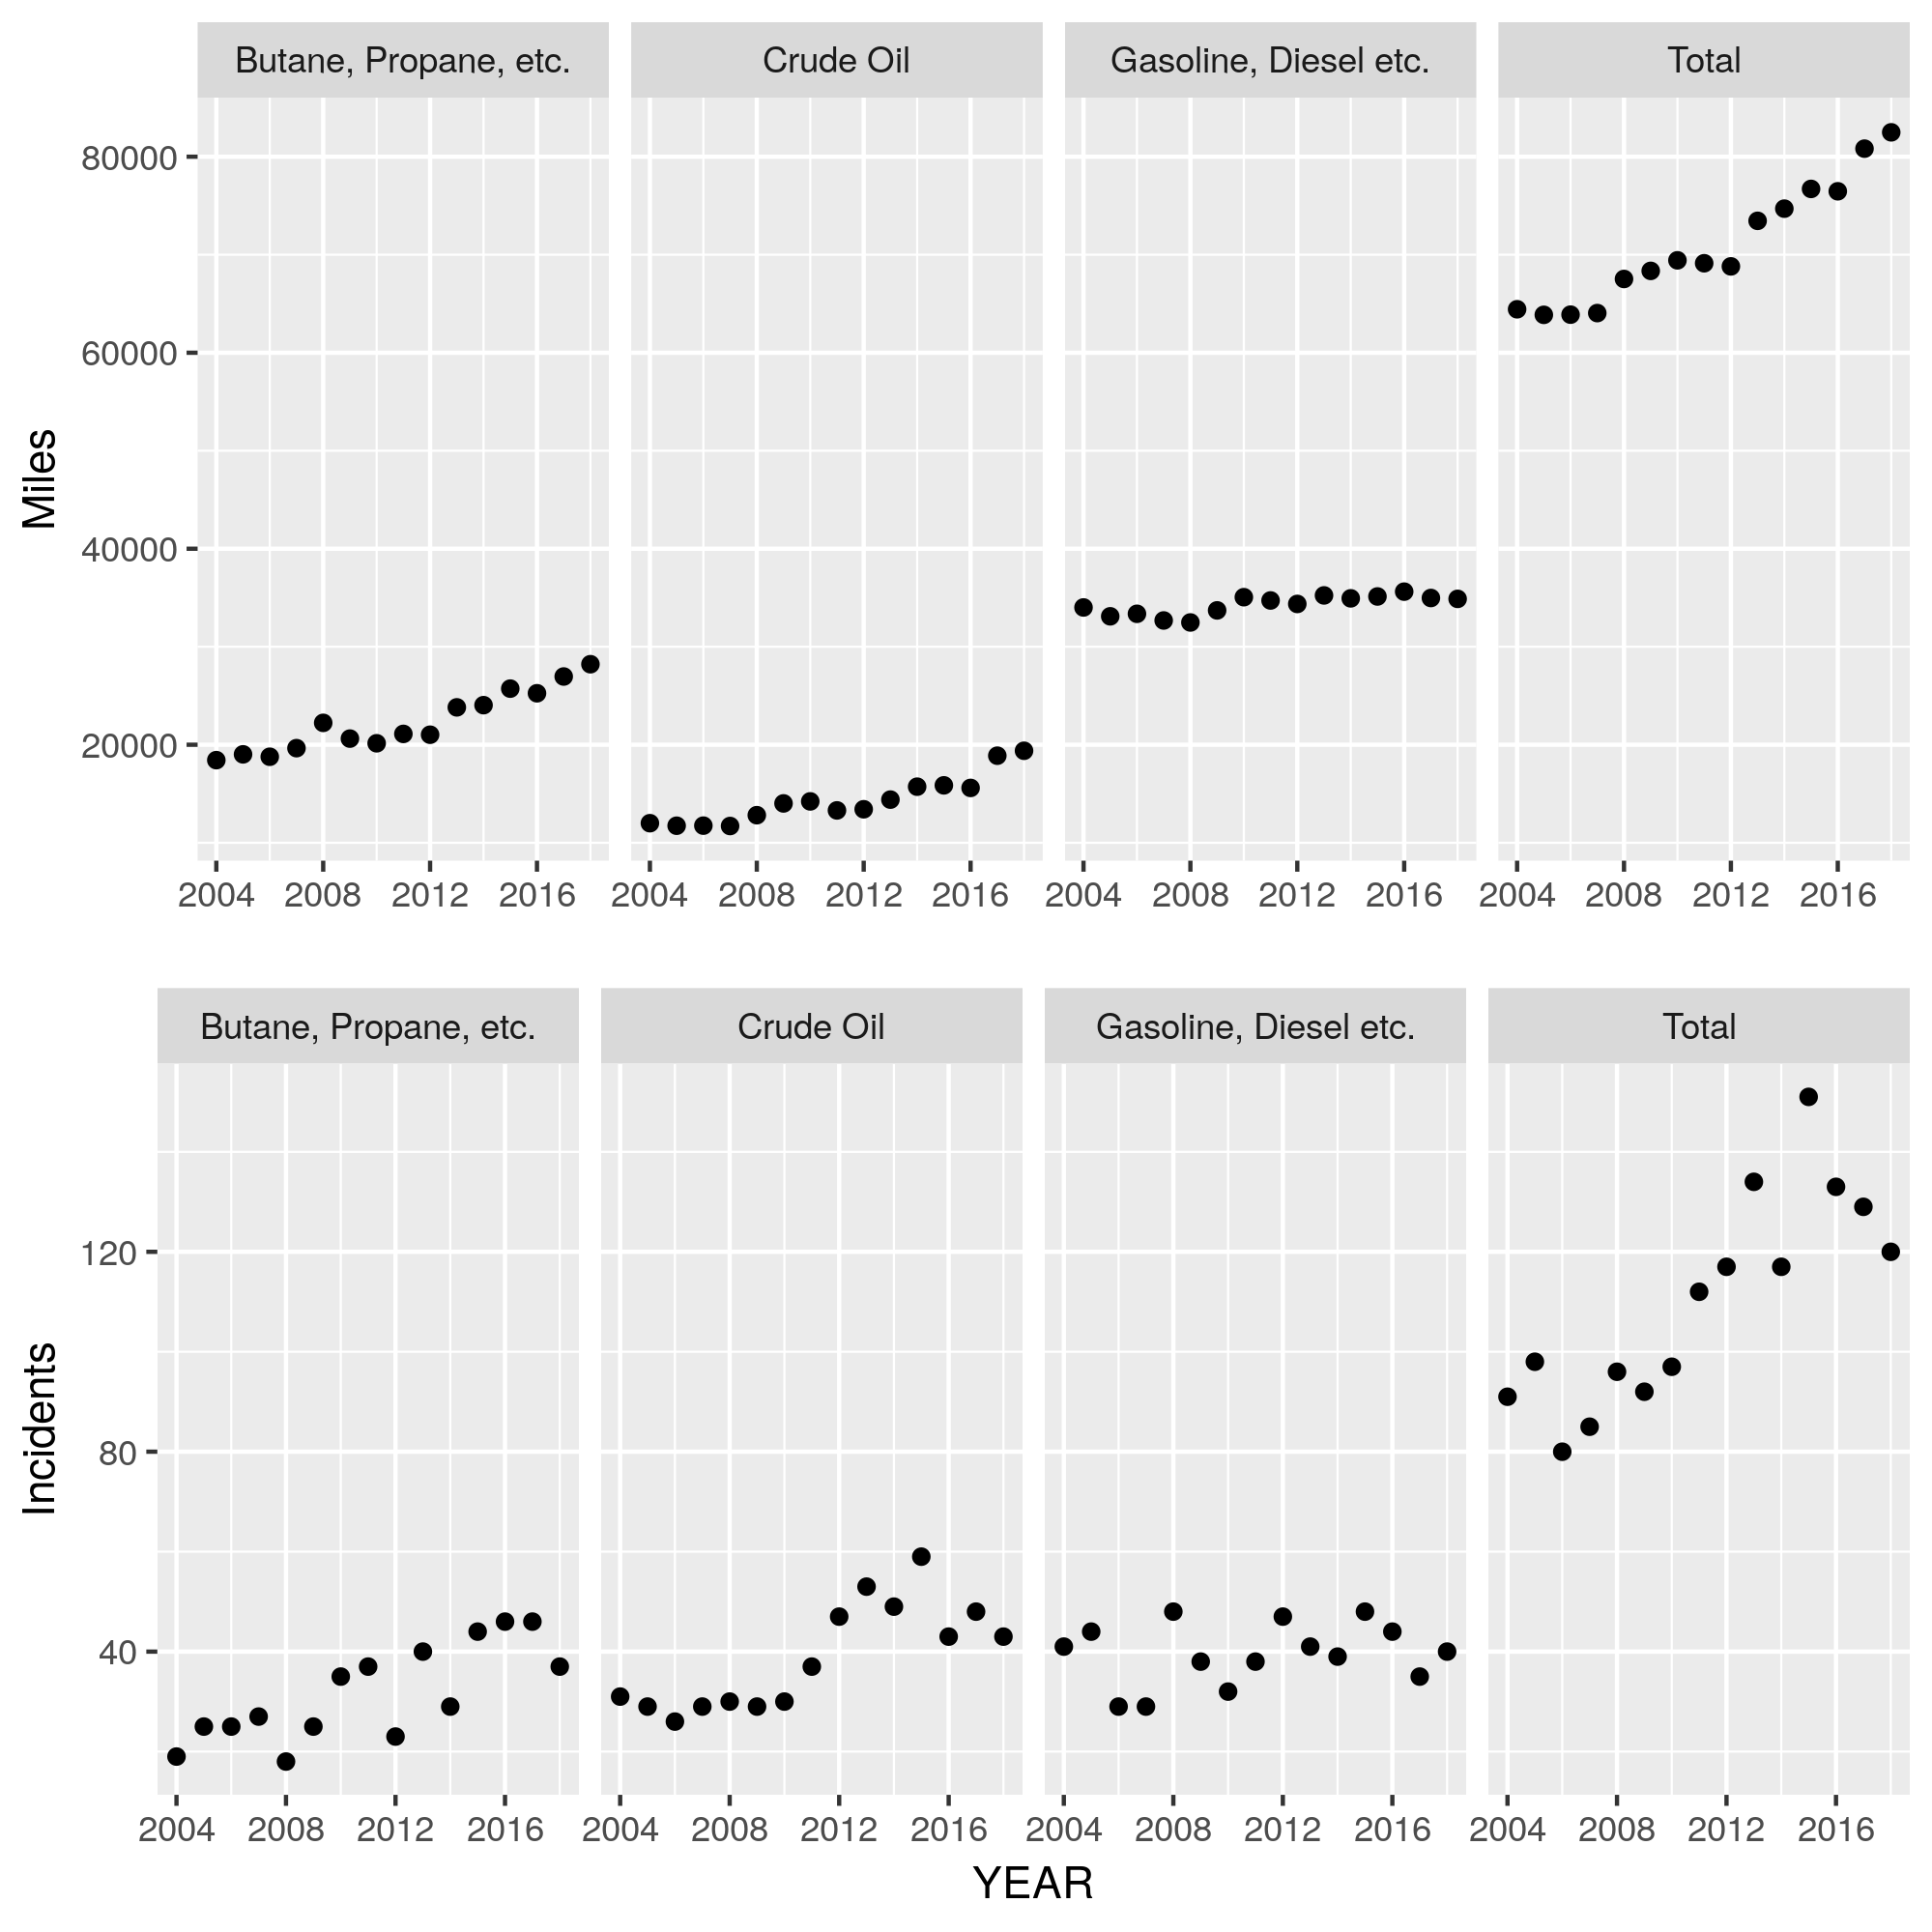
\includegraphics{illustrations/variables.png}
	\caption{}
\end{figure}

{\centering
	//////////////////////////////////////////////////////////////////////////////

	[Insert Figure 2 approximately here]

	//////////////////////////////////////////////////////////////////////////////\par
}

\begin{figure}
		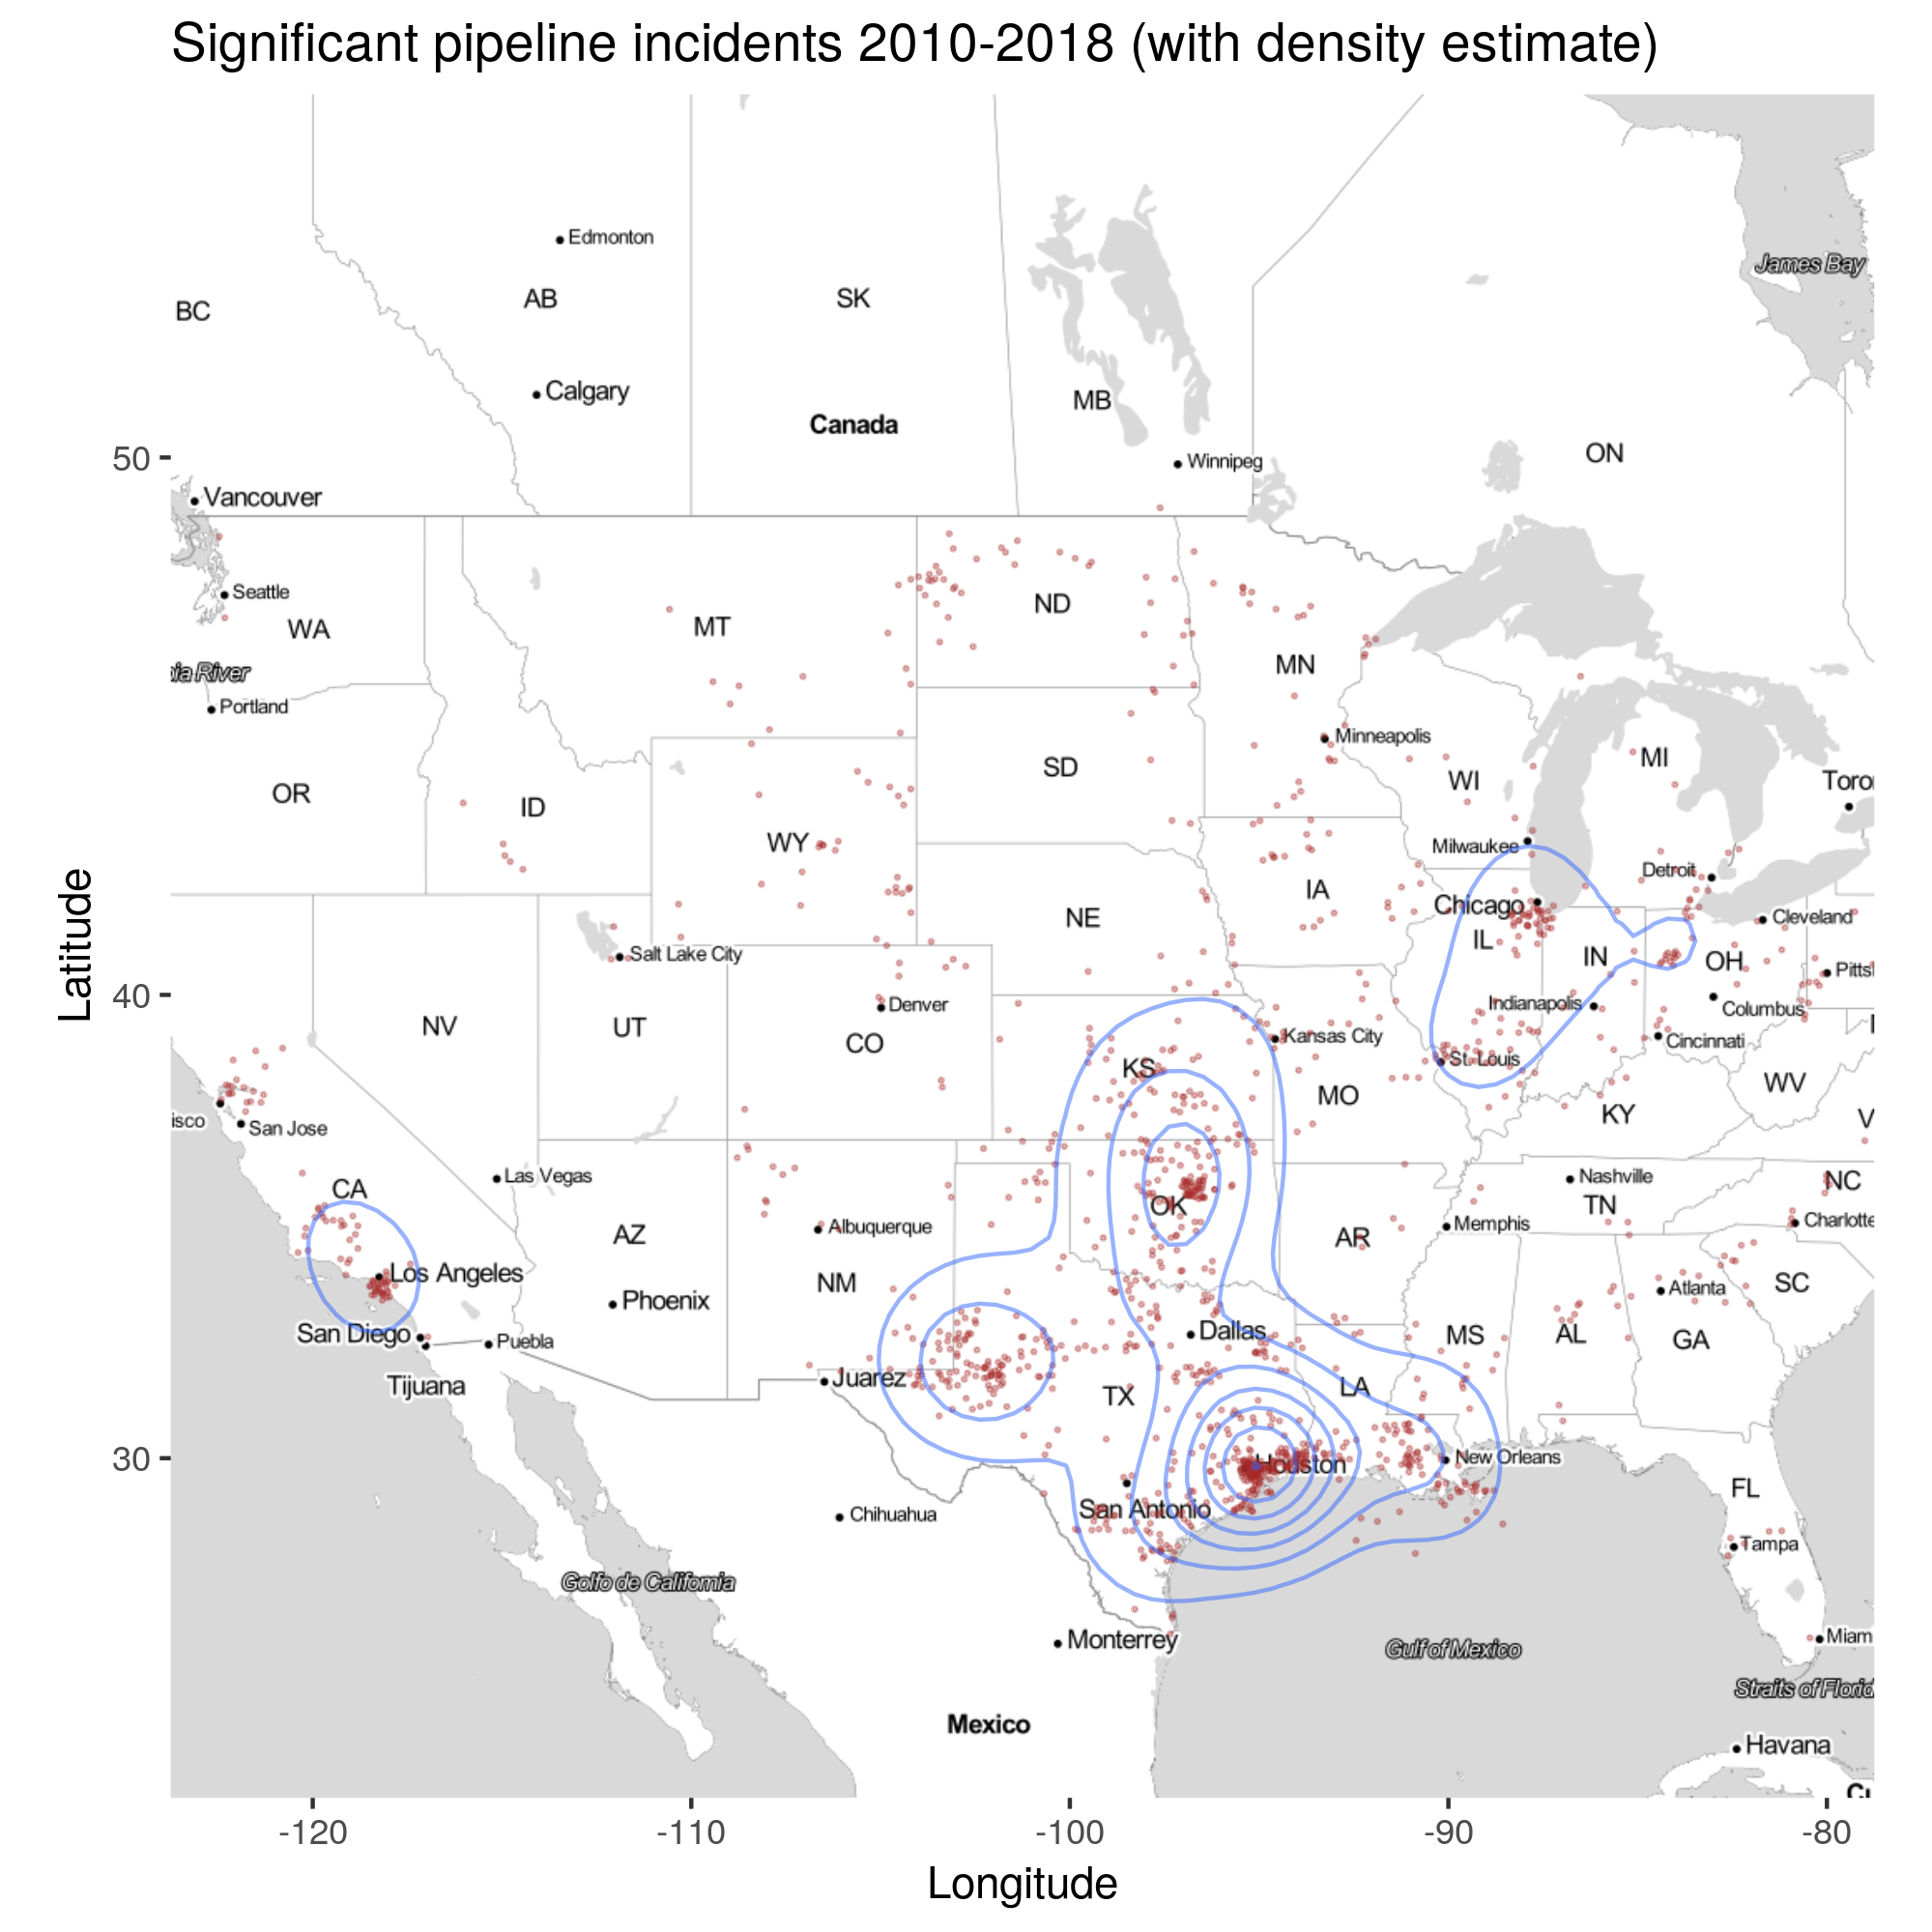
\includegraphics{illustrations/incidents.png}
		\caption{}
\end{figure}

The pipeline data has some shortcomings that we have addressed as well as possible. The data is not consolidated to the organization level. In many cases, for historic (M\&As) or legal reasons (joint ventures), even tightly controlled subsidiaries report their data separately. To address this issue, we selected the 200 largest observations in the data set (by peak pipeline miles per operator in any year of the observation period) and entered the legal names of these organizations into LexisNexis to retrieve the owners of the organziations. We also obtained from LexisNexis information on any past M\&A activities involving these organizations. We then conciliated the organizations to the group level where necessary, and used the resulting dataset for our analysis. Overall, 97 organizations belonged to 30 different company groups and we identified 7 separate M\&A events involving 6 different entities as reported by FERC, and 5 of the company groups that were identified by us. Four of the five largest operators in our sample are company groups that we have identified this way (see Figure 3). We have removed from the dataset information on CO2 pipelines (used for carbon capture and storage) and on biofuel pipelines: the definition and reporting of these pipeline types is not consistent between the reporting periods 2004-2009 and 2010-present, and the number of incidents related to these types of pipelines is low. We also did not include information on offshore pipelines in the dataset for the regression. Finally, we consolidated the incidents data to the organization level. We are controlling for the miles of pipelines for the three different commodities in the model; the residuals are the effects from organization effects that affect the pipeline network as a whole, regardless of the commodity transported: the effects of a pipeline management that successfully monitors pipelines, carries out maintenance, and reacts to stakeholder reports to prevent incidents (or fails to do any or all of that).

{\centering
	//////////////////////////////////////////////////////////////////////////////
	
	[Insert Figure 3 approximately here]
	
	//////////////////////////////////////////////////////////////////////////////\par
}

\begin{figure}
	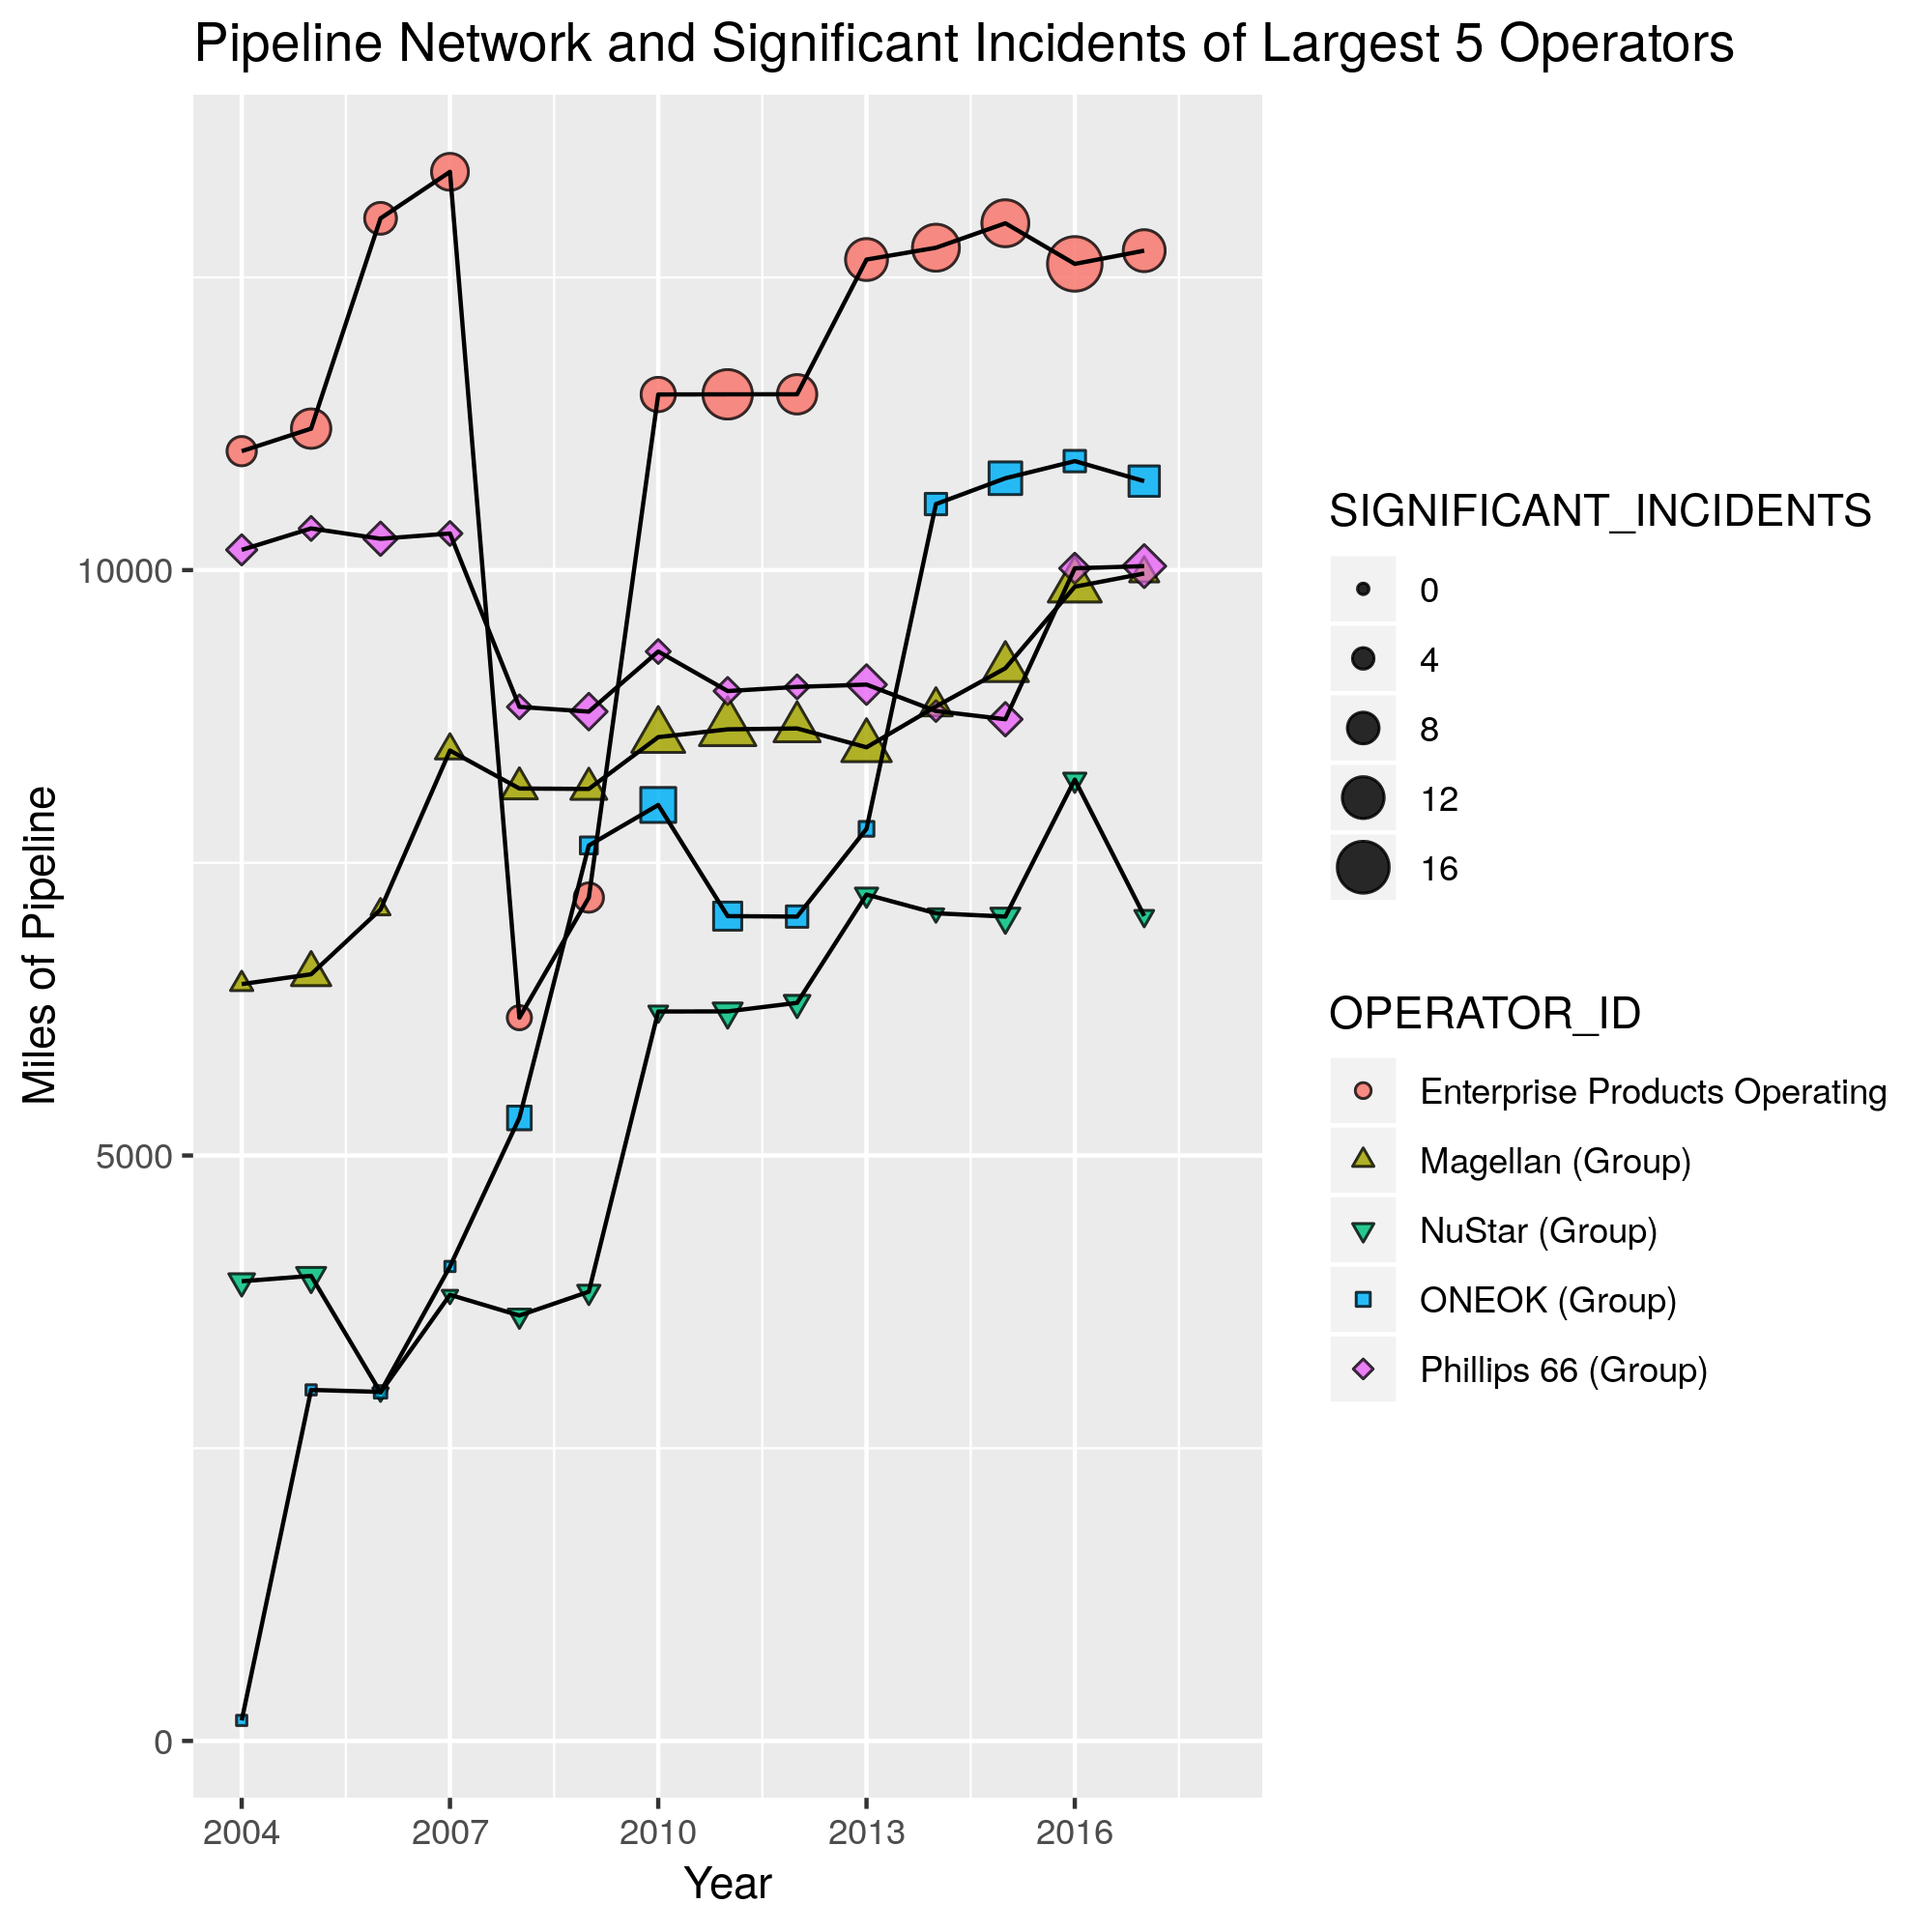
\includegraphics{illustrations/large_operators.png}
	\caption{}
\end{figure}

\subsection{Dependent variable}

We use the three-years moving average of significant pipeline incidents. A significant incident is one that either (1) caused an injury or fatality (2) \$50,000 in damage (in 1984 dollars), (3) involved the release of 5 barrels of liquid (or 50 barrels of gases such as Butane, Propane, etc.), or (4) led to an unintentional explosion or fire \citep{PHMSA}. Because the relationships described in this article play out over longer periods of time, a multi-year moving average of significant incidents ($i$) is a suitable modeling approach ($\bar{I} = (I_{t} + I_{t+1} + I_{t+2})/3$). As an added benefit, this approach further allowed us to calculate an independent variable that captures changes in strategy over a multi-year period; because the observations are only available as company-year data, we would not have been able to capture intra-year changes.

\subsection{Independent variable}

We capture both strategic adjustments, and phases of stability based on the changes that are being made to the pipeline network. To capture this, we calculate the year-over-year change $C$ (in percent) to the pipeline network $M$ ($C_{t} = M_{t} - M_{t-1}/M_{t-1}$) and then took the standard deviation of these values over a three-year period to obtain strategic adjustments $A$ ($A_{t} = ((C_{t} - \bar{C})^2 + (C_{t-1} - \bar{C})^2 + (C_{t-2} - \bar{C})^2) / 2$). In other words, a three-year period that saw no change to the extend of the pipeline network, or a steady increase, would have a very low value for strategic adjustments, whereas if an organization was to increases its pipeline network in the first year, \textit{abandons} some pipeline segments in the second year, and acquires new assets in the third year, this organization would yield a high value for strategic adjustments during that time period. Because the effect of adjustments or stability might grow exponentially the greater the change, and to test for the competing hypothesis H1c, we included a squared effect also.

\subsection{Control variables}

As mentioned above, we have to control for the miles of pipelines for each commodity to obtain accurate estimations. Every type of commodity has a slightly different base rate of incidents (see Figure 1), so we provide the average number of miles throughout the three year period that the DV is using. Further, there are multiple learning effects at play that we also want to control for. We control for technology by controlling for the age of the pipeline network. Models 1-3 use the average age of the pipeline network, as well as the interaction effect with the total miles of pipelines for each commodity. Models 4-6 provide more details to capture the effect of technology more precisely: these models use the number of miles constructed in each decade, for each commodity (e.g., in the year 2007, company x was operating y miles of crude pipeline originally constructed in the 1950, and y miles of crude pipeline constructed in the 1960, etc.). We are interested in the effect of strategic adjustments rather than the effects of consolidation. Whereas consolidation describes a company that is facing issues or attempts to raise its profitability by downsizing operations, strategic adjustment is a process of changing direction; we therefore constructed a measure for consolidation that measures the sell-off or abandonment of pipeline assets; this variable is added as an additional control variable in models 1, 3, 4, and 6. Further, we included control variables for M\&A events to control for some learning opportunities that may emerge from M\&As and improve pipeline safety. Finally, in addition to the control variable for pipeline age, we added in models 1, 3, 4, and 6 a control variable for pipelines miles added during the last four years, discounted for the current year, as well as t-2 and t-3: new technology will provide additional safety, and this effect is controlled for through the variables for pipeline network age -- but before new technology can exert this effect, the unfamiliar technology might exert a negative effect, while the staff familiarizes itself with the technology. This effect is distinct from the effect of adjustments and stability that we are interested in, and will occur regardless of whether changes are introduced gradually or abruptly. Finally, we included in models 1-3 control variables for there being no pipeline miles for a commodity, in order to control for a focus on one commodity, or a process of diversification. Finally, in models 3 and 6 we control for year effects.

\section{Results}

{\centering
	//////////////////////////////////////////////////////////////////////////////
	
	[Insert Table 1 approximately here]
	
	//////////////////////////////////////////////////////////////////////////////\par
}

\begin{table}
	\rotatebox{90}{
		\begin{minipage}{1.4 \textwidth}
			\begin{table}[H]
\centering
\resizebox{\linewidth}{!}{
\begin{tabular}{llllllllllllllllllllll}
\toprule
  & Mean & SD & Incidts & Adj. & Adj sq. & Miles add & Consolid. & MA & MA t-1 & Miles Crude & Age Crude & MxA Crude & M. HVL & A. HVL & MxA HVL & M. Non-HVL & A. Non-HVL & MxA Non-HVL & No Crude & No HVL & No Non-HVL\\
\midrule
Incidts & 4.71 & 7.68 & 1 &  &  &  &  &  &  &  &  &  &  &  &  &  &  &  &  &  & \\
Adj. & 0.16 & 0.59 & -0.06 & 1 &  &  &  &  &  &  &  &  &  &  &  &  &  &  &  &  & \\
Adj sq. & 0.38 & 2.62 & -0.06 & 0.93 & 1 &  &  &  &  &  &  &  &  &  &  &  &  &  &  &  & \\
Miles add & 0.25 & 0.41 & -0.04 & 0.31 & 0.16 & 1 &  &  &  &  &  &  &  &  &  &  &  &  &  &  & \\
Consolid. & 0.72 & 2.71 & -0.1 & 0.06 & -0.02 & 0.39 & 1 &  &  &  &  &  &  &  &  &  &  &  &  &  & \\
\addlinespace
MA & 0.02 & 0.14 & 0.19 & -0.02 & -0.02 & 0.01 & -0.02 & 1 &  &  &  &  &  &  &  &  &  &  &  &  & \\
MA t-1 & 0.02 & 0.14 & 0.19 & -0.03 & -0.02 & 0.02 & -0.02 & 0.24 & 1 &  &  &  &  &  &  &  &  &  &  &  & \\
Miles Crude & 541.85 & 1254.53 & 0.48 & -0.06 & -0.05 & -0.01 & -0.05 & 0.27 & 0.21 & 1 &  &  &  &  &  &  &  &  &  &  & \\
Age Crude & 21.03 & 19.99 & 0.07 & -0.11 & -0.09 & -0.04 & -0.15 & 0.03 & 0 & 0.32 & 1 &  &  &  &  &  &  &  &  &  & \\
MxA Crude & 20003.45 & 49261.14 & 0.45 & -0.06 & -0.05 & -0.01 & -0.05 & 0.28 & 0.11 & 0.98 & 0.36 & 1 &  &  &  &  &  &  &  &  & \\
\addlinespace
M. HVL & 954.78 & 2299.51 & 0.6 & -0.04 & -0.03 & -0.05 & -0.08 & 0 & 0.04 & -0.01 & -0.14 & -0.01 & 1 &  &  &  &  &  &  &  & \\
A. HVL & 19.81 & 17.91 & 0.27 & 0.09 & 0.08 & 0.05 & -0.06 & 0.09 & 0.11 & 0.17 & -0.13 & 0.16 & 0.29 & 1 &  &  &  &  &  &  & \\
MxA HVL & 30994.3 & 67449.59 & 0.61 & -0.03 & -0.02 & -0.05 & -0.08 & -0.01 & 0.05 & -0.01 & -0.11 & 0.01 & 0.99 & 0.34 & 1 &  &  &  &  &  & \\
M. Non-HVL & 1631.07 & 3280.34 & 0.57 & -0.08 & -0.05 & -0.08 & -0.1 & 0.05 & 0.03 & 0.15 & 0.13 & 0.16 & 0.25 & 0.2 & 0.31 & 1 &  &  &  &  & \\
A. Non-HVL & 23.37 & 18.76 & 0.33 & 0.02 & 0.03 & 0.01 & -0.11 & 0.03 & 0.01 & 0.12 & 0.06 & 0.12 & 0.23 & 0.2 & 0.24 & 0.39 & 1 &  &  &  & \\
\addlinespace
MxA Non-HVL & 67228.73 & 137336.75 & 0.58 & -0.07 & -0.04 & -0.07 & -0.09 & 0.05 & -0.01 & 0.11 & 0.12 & 0.14 & 0.26 & 0.2 & 0.28 & 0.98 & 0.41 & 1 &  &  & \\
No Crude & 0.39 & 0.49 & -0.07 & 0.15 & 0.14 & 0.01 & 0.16 & -0.06 & -0.07 & -0.35 & -0.8 & -0.33 & 0.15 & 0.13 & 0.13 & -0.05 & 0 & -0.01 & 1 &  & \\
No HVL & 0.38 & 0.49 & -0.29 & -0.12 & -0.1 & -0.14 & -0.07 & -0.11 & -0.12 & -0.16 & 0.26 & -0.16 & -0.33 & -0.84 & -0.36 & -0.18 & -0.18 & -0.2 & -0.29 & 1 & \\
No Non-HVL & 0.3 & 0.46 & -0.27 & 0.09 & 0.09 & 0.11 & 0.18 & -0.06 & -0.02 & -0.13 & 0.03 & -0.13 & -0.18 & -0.18 & -0.19 & -0.33 & -0.78 & -0.31 & 0.03 & 0.13 & 1\\
\bottomrule
\end{tabular}}
\end{table}

		\end{minipage}
	}
	\caption{}
\end{table}

{\centering
	//////////////////////////////////////////////////////////////////////////////
	
	[Insert Table 2 approximately here]
	
	//////////////////////////////////////////////////////////////////////////////\par
}

\begin{table}
	\rotatebox{90}{
		\begin{minipage}{1.4 \textwidth}
			\begin{table}[H]
\centering
\resizebox{\linewidth}{!}{
\begin{tabular}{llllllllllllllllllllllllllllllllll}
\toprule
  & Mean & SD & Incidts & Adj. & Adj sq. & Miles add & Consolid. & MA & MA t-1 & Crude 40s & Crude 50s & Crude 60s & Crude 70s & Crude 80s & Crude 90s & Crude 00s & Crude 10s & HVL 40s & HVL 50s & HVL 60s & HVL 70s & HVL 80s & HVL 90s & HLV 00s & HVL 10s & Non-HVL 40s & Non-HVL 50s & Non-HVL 60s & Non-HVL 70s & Non-HVL 80s & Non-HVL 90s & Non-HVL 00s & Non-HVL 10s\\
\midrule
Incidts & 4.71 & 7.68 & 1 &  &  &  &  &  &  &  &  &  &  &  &  &  &  &  &  &  &  &  &  &  &  &  &  &  &  &  &  &  & \\
Adj. & 0.16 & 0.59 & -0.06 & 1 &  &  &  &  &  &  &  &  &  &  &  &  &  &  &  &  &  &  &  &  &  &  &  &  &  &  &  &  & \\
Adj sq. & 0.38 & 2.62 & -0.06 & 0.93 & 1 &  &  &  &  &  &  &  &  &  &  &  &  &  &  &  &  &  &  &  &  &  &  &  &  &  &  &  & \\
Miles add & 0.25 & 0.41 & -0.04 & 0.31 & 0.16 & 1 &  &  &  &  &  &  &  &  &  &  &  &  &  &  &  &  &  &  &  &  &  &  &  &  &  &  & \\
Consolid. & 0.72 & 2.71 & -0.1 & 0.06 & -0.02 & 0.39 & 1 &  &  &  &  &  &  &  &  &  &  &  &  &  &  &  &  &  &  &  &  &  &  &  &  &  & \\
\addlinespace
MA & 0.02 & 0.14 & 0.19 & -0.02 & -0.02 & 0.01 & -0.02 & 1 &  &  &  &  &  &  &  &  &  &  &  &  &  &  &  &  &  &  &  &  &  &  &  &  & \\
MA t-1 & 0.02 & 0.14 & 0.19 & -0.03 & -0.02 & 0.02 & -0.02 & 0.24 & 1 &  &  &  &  &  &  &  &  &  &  &  &  &  &  &  &  &  &  &  &  &  &  &  & \\
Crude 40s & 90.48 & 283.05 & 0.23 & -0.06 & -0.04 & -0.06 & -0.06 & 0.11 & 0.08 & 1 &  &  &  &  &  &  &  &  &  &  &  &  &  &  &  &  &  &  &  &  &  &  & \\
Crude 50s & 196.52 & 465.59 & 0.33 & -0.09 & -0.06 & -0.07 & -0.07 & 0.14 & 0.08 & 0.71 & 1 &  &  &  &  &  &  &  &  &  &  &  &  &  &  &  &  &  &  &  &  &  & \\
Crude 60s & 111.21 & 332.14 & 0.35 & -0.07 & -0.04 & -0.06 & -0.06 & 0.17 & 0.13 & 0.78 & 0.69 & 1 &  &  &  &  &  &  &  &  &  &  &  &  &  &  &  &  &  &  &  &  & \\
\addlinespace
Crude 70s & 88.78 & 188.15 & 0.14 & -0.09 & -0.06 & -0.09 & -0.08 & 0.01 & -0.01 & 0.06 & 0.33 & 0.25 & 1 &  &  &  &  &  &  &  &  &  &  &  &  &  &  &  &  &  &  &  & \\
Crude 80s & 80.42 & 358.7 & 0.05 & -0.05 & -0.03 & -0.06 & -0.05 & -0.01 & -0.01 & 0.07 & 0.19 & 0.05 & 0.52 & 1 &  &  &  &  &  &  &  &  &  &  &  &  &  &  &  &  &  &  & \\
Crude 90s & 141.19 & 450.95 & 0.25 & -0.06 & -0.04 & -0.08 & -0.05 & 0.3 & 0.18 & 0.54 & 0.47 & 0.53 & 0.13 & 0.1 & 1 &  &  &  &  &  &  &  &  &  &  &  &  &  &  &  &  &  & \\
Crude 00s & 67.36 & 200.6 & 0.1 & -0.06 & -0.04 & -0.05 & -0.04 & 0.04 & 0.04 & 0.2 & 0.28 & 0.23 & 0.27 & 0.41 & 0.29 & 1 &  &  &  &  &  &  &  &  &  &  &  &  &  &  &  &  & \\
Crude 10s & 32.24 & 122.97 & 0.16 & -0.04 & -0.03 & -0.05 & -0.03 & -0.02 & 0.09 & 0.01 & 0.11 & 0.08 & 0.26 & 0.07 & 0.06 & 0.27 & 1 &  &  &  &  &  &  &  &  &  &  &  &  &  &  &  & \\
\addlinespace
HVL 40s & 49.73 & 164.69 & 0.39 & -0.05 & -0.03 & -0.03 & -0.06 & -0.02 & 0.07 & 0.49 & 0.5 & 0.49 & 0.04 & 0 & 0.01 & -0.04 & 0.05 & 1 &  &  &  &  &  &  &  &  &  &  &  &  &  &  & \\
HVL 50s & 148.2 & 422.6 & 0.32 & 0.03 & 0 & 0.02 & -0.07 & 0.1 & 0.12 & 0.32 & 0.33 & 0.32 & -0.01 & -0.01 & 0.1 & -0.02 & -0.02 & 0.47 & 1 &  &  &  &  &  &  &  &  &  &  &  &  &  & \\
HVL 60s & 512.26 & 1455.51 & 0.57 & 0 & -0.02 & -0.01 & -0.06 & -0.02 & 0 & 0.03 & 0.06 & 0.05 & -0.02 & -0.01 & -0.02 & -0.04 & 0 & 0.56 & 0.37 & 1 &  &  &  &  &  &  &  &  &  &  &  &  & \\
HVL 70s & 511.79 & 1069.86 & 0.47 & 0.02 & 0.01 & -0.03 & -0.1 & -0.03 & -0.04 & 0.05 & 0.13 & 0.05 & -0.06 & -0.05 & 0.03 & -0.1 & 0.07 & 0.48 & 0.43 & 0.68 & 1 &  &  &  &  &  &  &  &  &  &  &  & \\
HVL 80s & 244.6 & 909.02 & 0.48 & 0 & -0.02 & 0 & -0.04 & -0.02 & -0.03 & 0.01 & -0.01 & -0.02 & -0.04 & 0.06 & -0.06 & -0.03 & -0.04 & 0.45 & 0.22 & 0.87 & 0.7 & 1 &  &  &  &  &  &  &  &  &  &  & \\
\addlinespace
HVL 90s & 294.94 & 1008.73 & 0.51 & -0.01 & -0.02 & -0.01 & -0.05 & 0 & -0.02 & 0.1 & 0.08 & 0.09 & -0.08 & -0.02 & 0 & -0.06 & -0.06 & 0.53 & 0.28 & 0.87 & 0.71 & 0.96 & 1 &  &  &  &  &  &  &  &  &  & \\
HLV 00s & 136.4 & 531.01 & 0.35 & -0.03 & -0.03 & -0.01 & -0.02 & -0.01 & 0 & -0.07 & -0.07 & -0.07 & -0.1 & -0.05 & -0.07 & -0.08 & -0.05 & 0.26 & 0.19 & 0.64 & 0.51 & 0.69 & 0.66 & 1 &  &  &  &  &  &  &  &  & \\
HVL 10s & 67.38 & 407.69 & 0.29 & -0.04 & -0.02 & -0.04 & -0.02 & 0.05 & 0.19 & -0.02 & -0.02 & -0.01 & -0.05 & -0.03 & -0.04 & -0.04 & 0.05 & 0.2 & 0.27 & 0.26 & 0.3 & 0.36 & 0.37 & 0.34 & 1 &  &  &  &  &  &  &  & \\
Non-HVL 40s & 154.34 & 597.85 & 0.36 & -0.03 & -0.02 & -0.03 & -0.05 & 0 & -0.02 & -0.03 & 0.03 & 0.02 & 0.07 & -0.05 & -0.06 & -0.07 & 0.05 & 0.04 & 0.12 & 0.1 & 0.11 & -0.01 & 0.02 & -0.01 & -0.02 & 1 &  &  &  &  &  &  & \\
Non-HVL 50s & 430.49 & 1282.41 & 0.44 & -0.05 & -0.03 & -0.03 & -0.07 & 0.01 & 0 & 0.17 & 0.25 & 0.24 & 0.14 & -0.01 & 0.03 & -0.04 & 0.12 & 0.24 & 0.31 & 0.15 & 0.26 & 0 & 0.05 & -0.01 & -0.02 & 0.87 & 1 &  &  &  &  &  & \\
\addlinespace
Non-HVL 60s & 435.28 & 1049.93 & 0.51 & -0.09 & -0.05 & -0.08 & -0.09 & 0.02 & 0.01 & 0.14 & 0.29 & 0.17 & 0.1 & -0.04 & 0.11 & -0.03 & 0.13 & 0.21 & 0.2 & 0.09 & 0.38 & 0.01 & 0.06 & 0.02 & -0.03 & 0.5 & 0.61 & 1 &  &  &  &  & \\
Non-HVL 70s & 305.52 & 665.39 & 0.52 & -0.1 & -0.06 & -0.09 & -0.1 & 0.08 & 0.05 & 0.06 & 0.17 & 0.11 & 0.08 & -0.07 & 0.03 & -0.09 & 0.12 & 0.26 & 0.1 & 0.27 & 0.34 & 0.2 & 0.25 & 0.07 & 0.05 & 0.51 & 0.6 & 0.65 & 1 &  &  &  & \\
Non-HVL 80s & 174.22 & 503.67 & 0.33 & -0.07 & -0.04 & -0.08 & -0.08 & -0.01 & 0 & 0.26 & 0.5 & 0.25 & 0.42 & 0.61 & 0.1 & 0.22 & 0.16 & 0.38 & 0.21 & 0.12 & 0.36 & 0.13 & 0.12 & 0.01 & -0.03 & 0.04 & 0.23 & 0.55 & 0.35 & 1 &  &  & \\
Non-HVL 90s & 200.85 & 562.18 & 0.21 & -0.07 & -0.04 & -0.1 & -0.07 & 0.12 & 0.11 & 0.15 & 0.31 & 0.19 & 0.25 & 0.24 & 0.35 & 0.11 & 0.2 & 0.2 & 0.14 & 0.08 & 0.33 & 0.01 & 0.04 & -0.04 & -0.04 & 0.19 & 0.43 & 0.43 & 0.42 & 0.53 & 1 &  & \\
Non-HVL 00s & 119.97 & 313.53 & 0.43 & -0.09 & -0.05 & -0.08 & -0.09 & 0.19 & 0.11 & 0.46 & 0.67 & 0.45 & 0.19 & -0.02 & 0.45 & 0.13 & 0.16 & 0.34 & 0.25 & 0.07 & 0.34 & 0 & 0.07 & -0.02 & -0.04 & 0.27 & 0.47 & 0.63 & 0.49 & 0.52 & 0.49 & 1 & \\
\addlinespace
Non-HVL 10s & 14.97 & 100.05 & 0.06 & -0.04 & -0.02 & -0.02 & -0.02 & -0.02 & 0.01 & 0.06 & 0.09 & 0.08 & 0.01 & 0.02 & 0.02 & 0.15 & 0.05 & 0.08 & 0.06 & 0 & 0.01 & -0.01 & 0 & -0.01 & 0.05 & 0 & 0.08 & 0.06 & 0 & 0.09 & 0.18 & 0.12 & 1\\
\bottomrule
\end{tabular}}
\end{table}

		\end{minipage}
	}
	\caption{}
\end{table}

We ran a fixed effects model with clustered standard errors to estimate the effects. Before selecting that model specification, we also ran a Hausman test to ensure that a fixed effects model is an appropriate choice. The linear effect of adjustments is significant at the 0.1 confidence level for models 2, 4,5, and 6, whereas the squared effect is significant at the 0.1 confidence interval only for model 2. For the other models, the standard error does place the results close to the 0.1 confidence level also (see Table 3 and Table 4). To get an impression of the effect of the adjustment variable at above and below 0, we plotted out both the linear and squared effect for model 2, which would show the most easily interpretable trend due to the significance level of both the the linear and squared effect (see Figure 4) -- the results may not be generalizable, as the squared effect is not significant in the other models. The clear negative trend for negative values implies that when a company enters a phase of stability, the rate of significant incidents does decrease, supporting \textit{Hypothesis 2}. For the positive range, which describes an uptick in strategic adjustments, the 95\% confidence interval includes both positive and negative values -- there is no clear evidence that these adjustments from the parent organizations disrupt or setback the learning toward pipeline safety. \textit{Hypothesis 1} does not have clear support. On the other hand, the results also do not allow us to conclude that strategic adjustments act as shocks that facilitate additional learning (competing \textit{Hypothesis 1c}).

{\centering
	//////////////////////////////////////////////////////////////////////////////
	
	[Insert Table 3 approximately here]
	
	//////////////////////////////////////////////////////////////////////////////\par
}

\begin{table}
	{\renewcommand\normalsize{\tiny}%
		\normalsize
	\begin{tabular}{llll}
\toprule
{} &                        Model 1 &                         Model 2 &                         Model 3 \\
\midrule
Adjustments         &       $\makecell{1.5\\(1.21)}$ &   $\makecell{1.93^{*}\\(1.15)}$ &       $\makecell{1.41\\(1.19)}$ \\
Adjustments sq.     &     $\makecell{-0.46\\(0.33)}$ &  $\makecell{-0.54^{*}\\(0.31)}$ &      $\makecell{-0.42\\(0.32)}$ \\
Miles add           &      $\makecell{0.17\\(0.59)}$ &                                 &        $\makecell{0.1\\(0.59)}$ \\
Consolidation       &       $\makecell{0.07\\(0.1)}$ &                                 &        $\makecell{0.08\\(0.1)}$ \\
M and A             &      $\makecell{1.53\\(1.92)}$ &  $\makecell{3.75^{**}\\(1.64)}$ &       $\makecell{1.75\\(2.02)}$ \\
M and A t-1         &     $\makecell{-1.58\\(1.14)}$ &      $\makecell{-1.21\\(0.83)}$ &      $\makecell{-1.36\\(1.16)}$ \\
Miles Crude         &        $\makecell{0.0\\(0.0)}$ &         $\makecell{0.0\\(0.0)}$ &         $\makecell{0.0\\(0.0)}$ \\
Age Crude           &  $\makecell{0.04^{*}\\(0.02)}$ &       $\makecell{0.01\\(0.02)}$ &   $\makecell{0.04^{*}\\(0.02)}$ \\
Miles x Age Crude   &       $\makecell{-0.0\\(0.0)}$ &   $\makecell{-0.0^{**}\\(0.0)}$ &        $\makecell{-0.0\\(0.0)}$ \\
Miles HVL           &      $\makecell{0.01\\(0.01)}$ &        $\makecell{0.0\\(0.01)}$ &       $\makecell{0.01\\(0.01)}$ \\
Age HVL             &      $\makecell{0.04\\(0.03)}$ &   $\makecell{0.04^{*}\\(0.03)}$ &       $\makecell{0.04\\(0.03)}$ \\
Miles x Age HVL     &       $\makecell{-0.0\\(0.0)}$ &        $\makecell{-0.0\\(0.0)}$ &        $\makecell{-0.0\\(0.0)}$ \\
Miles Non-HVL       &        $\makecell{0.0\\(0.0)}$ &         $\makecell{0.0\\(0.0)}$ &         $\makecell{0.0\\(0.0)}$ \\
Age Non-HVL         &      $\makecell{-0.0\\(0.03)}$ &        $\makecell{0.0\\(0.02)}$ &      $\makecell{-0.01\\(0.03)}$ \\
Miles x Age Non-HVL &       $\makecell{-0.0\\(0.0)}$ &        $\makecell{-0.0\\(0.0)}$ &        $\makecell{-0.0\\(0.0)}$ \\
No Crude            &  $\makecell{-8.66^{*}\\(4.5)}$ &      $\makecell{-1.78\\(2.71)}$ &  $\makecell{-8.63^{*}\\(4.39)}$ \\
No HVL              &      $\makecell{1.68\\(1.22)}$ &       $\makecell{0.98\\(0.85)}$ &       $\makecell{1.69\\(1.32)}$ \\
No Non-HVL          &     $\makecell{-3.19\\(2.94)}$ &       $\makecell{-1.59\\(2.4)}$ &      $\makecell{-2.87\\(3.02)}$ \\
2007                &                                &                                 &      $\makecell{-0.19\\(0.38)}$ \\
2008                &                                &                                 &       $\makecell{0.03\\(0.57)}$ \\
2009                &                                &                                 &        $\makecell{0.3\\(0.65)}$ \\
2010                &                                &                                 &        $\makecell{0.43\\(0.7)}$ \\
2011                &                                &                                 &       $\makecell{0.44\\(0.62)}$ \\
2012                &                                &                                 &       $\makecell{0.56\\(0.69)}$ \\
Constant            &      $\makecell{2.12\\(2.42)}$ &      $\makecell{-1.83\\(2.42)}$ &       $\makecell{1.89\\(2.39)}$ \\
Groups              &                             69 &                              70 &                              69 \\
Observations        &                            401 &                             474 &                             401 \\
R-sq within         &                           0.33 &                            0.32 &                            0.33 \\
R-sq between        &                            0.3 &                            0.43 &                             0.3 \\
R-sq overall        &                           0.34 &                            0.42 &                            0.33 \\
\bottomrule
*: Significant at the 0.9 level. & **: Significant at the 0.95 level. & ***: Significant at the 0.99 level.
\end{tabular}
}
	\caption{}
\end{table}

{\centering
	//////////////////////////////////////////////////////////////////////////////
	
	[Insert Table 4 approximately here]
	
	//////////////////////////////////////////////////////////////////////////////\par
}

\begin{table}
	{\renewcommand\normalsize{\tiny}%
		\normalsize
		\begin{tabular}{ll}

\begin{tabular}{llll}
\toprule
{} &                           Model 4 &                          Model 5 &                           Model 6 \\
\midrule
Adjustments         &     $\makecell{1.22^{*}\\(0.65)}$ &    $\makecell{1.29^{*}\\(0.77)}$ &     $\makecell{1.24^{*}\\(0.66)}$ \\
Adjustments sq.     &        $\makecell{-0.22\\(0.14)}$ &       $\makecell{-0.26\\(0.17)}$ &        $\makecell{-0.21\\(0.14)}$ \\
Miles add           &    $\makecell{-0.57^{*}\\(0.33)}$ &                                  &        $\makecell{-0.48\\(0.32)}$ \\
Consolidation       &    $\makecell{0.1^{***}\\(0.03)}$ &                                  &   $\makecell{0.09^{***}\\(0.03)}$ \\
M and A             &         $\makecell{2.22\\(1.45)}$ &  $\makecell{2.31^{***}\\(0.79)}$ &          $\makecell{2.47\\(1.5)}$ \\
M and A t-1         &  $\makecell{-0.89^{***}\\(0.28)}$ &        $\makecell{1.15\\(0.77)}$ &   $\makecell{-0.96^{**}\\(0.44)}$ \\
Miles Crude 1940s   &          $\makecell{-0.0\\(0.0)}$ &         $\makecell{-0.0\\(0.0)}$ &           $\makecell{0.0\\(0.0)}$ \\
Miles Crude 1950s   &    $\makecell{0.01^{***}\\(0.0)}$ &      $\makecell{0.0^{*}\\(0.0)}$ &    $\makecell{0.01^{***}\\(0.0)}$ \\
Miles Crude 1960s   &         $\makecell{0.01\\(0.01)}$ &          $\makecell{0.0\\(0.0)}$ &         $\makecell{0.01\\(0.01)}$ \\
Miles Crude 1970s   &           $\makecell{0.0\\(0.0)}$ &          $\makecell{0.0\\(0.0)}$ &           $\makecell{0.0\\(0.0)}$ \\
Miles Crude 1980s   &         $\makecell{0.01\\(0.01)}$ &        $\makecell{0.01\\(0.01)}$ &         $\makecell{0.01\\(0.01)}$ \\
Miles Crude 1990s   &           $\makecell{0.0\\(0.0)}$ &          $\makecell{0.0\\(0.0)}$ &           $\makecell{0.0\\(0.0)}$ \\
Miles Crude 2000s   &          $\makecell{-0.0\\(0.0)}$ &      $\makecell{0.0^{*}\\(0.0)}$ &          $\makecell{-0.0\\(0.0)}$ \\
Miles Crude 2010s   &         $\makecell{-0.0\\(0.01)}$ &          $\makecell{0.0\\(0.0)}$ &          $\makecell{0.0\\(0.01)}$ \\
Miles HVL 1940s     &        $\makecell{-0.01\\(0.01)}$ &         $\makecell{0.0\\(0.01)}$ &        $\makecell{-0.01\\(0.01)}$ \\
Miles HVL 1950s     &          $\makecell{-0.0\\(0.0)}$ &          $\makecell{0.0\\(0.0)}$ &          $\makecell{-0.0\\(0.0)}$ \\
Miles HVL 1960s     &      $\makecell{0.0^{**}\\(0.0)}$ &     $\makecell{0.0^{**}\\(0.0)}$ &      $\makecell{0.0^{**}\\(0.0)}$ \\
Miles HVL 1970s     &    $\makecell{-0.0^{***}\\(0.0)}$ &   $\makecell{-0.0^{***}\\(0.0)}$ &    $\makecell{-0.0^{***}\\(0.0)}$ \\
Miles HVL 1980s     &          $\makecell{-0.0\\(0.0)}$ &         $\makecell{-0.0\\(0.0)}$ &           $\makecell{0.0\\(0.0)}$ \\
Miles HVL 1990s     &           $\makecell{0.0\\(0.0)}$ &     $\makecell{0.0^{**}\\(0.0)}$ &           $\makecell{0.0\\(0.0)}$ \\
Miles HVL 2000s     &      $\makecell{0.0^{**}\\(0.0)}$ &          $\makecell{0.0\\(0.0)}$ &      $\makecell{0.0^{**}\\(0.0)}$ \\
Miles HVL 2010s     &    $\makecell{0.02^{**}\\(0.01)}$ &          $\makecell{0.0\\(0.0)}$ &    $\makecell{0.02^{**}\\(0.01)}$ \\
\bottomrule
cont.
\end{tabular}

\begin{tabular}{llll}
\toprule
{} &                           Model 4 &                          Model 5 &                           Model 6 \\
\midrule
Miles Non-HVL 1940s &   $\makecell{-0.01^{***}\\(0.0)}$ &   $\makecell{-0.0^{***}\\(0.0)}$ &   $\makecell{-0.01^{***}\\(0.0)}$ \\
Miles Non-HVL 1950s &          $\makecell{-0.0\\(0.0)}$ &          $\makecell{0.0\\(0.0)}$ &          $\makecell{-0.0\\(0.0)}$ \\
Miles Non-HVL 1960s &           $\makecell{0.0\\(0.0)}$ &          $\makecell{0.0\\(0.0)}$ &           $\makecell{0.0\\(0.0)}$ \\
Miles Non-HVL 1970s &           $\makecell{0.0\\(0.0)}$ &          $\makecell{0.0\\(0.0)}$ &           $\makecell{0.0\\(0.0)}$ \\
Miles Non-HVL 1980s &    $\makecell{0.02^{***}\\(0.0)}$ &   $\makecell{0.02^{***}\\(0.0)}$ &    $\makecell{0.02^{***}\\(0.0)}$ \\
Miles Non-HVL 1990s &          $\makecell{0.0\\(0.01)}$ &        $\makecell{-0.0\\(0.01)}$ &          $\makecell{0.0\\(0.01)}$ \\
Miles Non-HVL 2000s &          $\makecell{-0.0\\(0.0)}$ &         $\makecell{-0.0\\(0.0)}$ &          $\makecell{-0.0\\(0.0)}$ \\
Miles Non-HVL 2010s &           $\makecell{0.0\\(0.0)}$ &     $\makecell{0.01^{*}\\(0.0)}$ &           $\makecell{0.0\\(0.0)}$ \\
2007                &                                   &                                  &         $\makecell{-0.3\\(0.32)}$ \\
2008                &                                   &                                  &         $\makecell{0.02\\(0.35)}$ \\
2009                &                                   &                                  &         $\makecell{0.24\\(0.47)}$ \\
2010                &                                   &                                  &         $\makecell{0.13\\(0.52)}$ \\
2011                &                                   &                                  &        $\makecell{-0.29\\(0.48)}$ \\
2012                &                                   &                                  &        $\makecell{-0.53\\(0.59)}$ \\
Constant            &  $\makecell{-4.21^{***}\\(1.11)}$ &  $\makecell{-2.88^{**}\\(1.23)}$ &  $\makecell{-4.21^{***}\\(1.08)}$ \\
Groups              &                                69 &                               78 &                                69 \\
Observations        &                               401 &                              624 &                               401 \\
R-sq within         &                              0.75 &                             0.62 &                              0.76 \\
R-sq between        &                               0.2 &                              0.3 &                              0.19 \\
R-sq overall        &                              0.21 &                              0.3 &                               0.2 \\
\bottomrule
*: Significant at the 0.9 level. & **: Significant at the 0.95 level. & ***: Significant at the 0.99 level.
\end{tabular}

\end{tabular}}
	\caption{}
\end{table}

{\centering
	//////////////////////////////////////////////////////////////////////////////
	
	[Insert Figure 4 approximately here]
	
	//////////////////////////////////////////////////////////////////////////////\par
}

\begin{figure}
	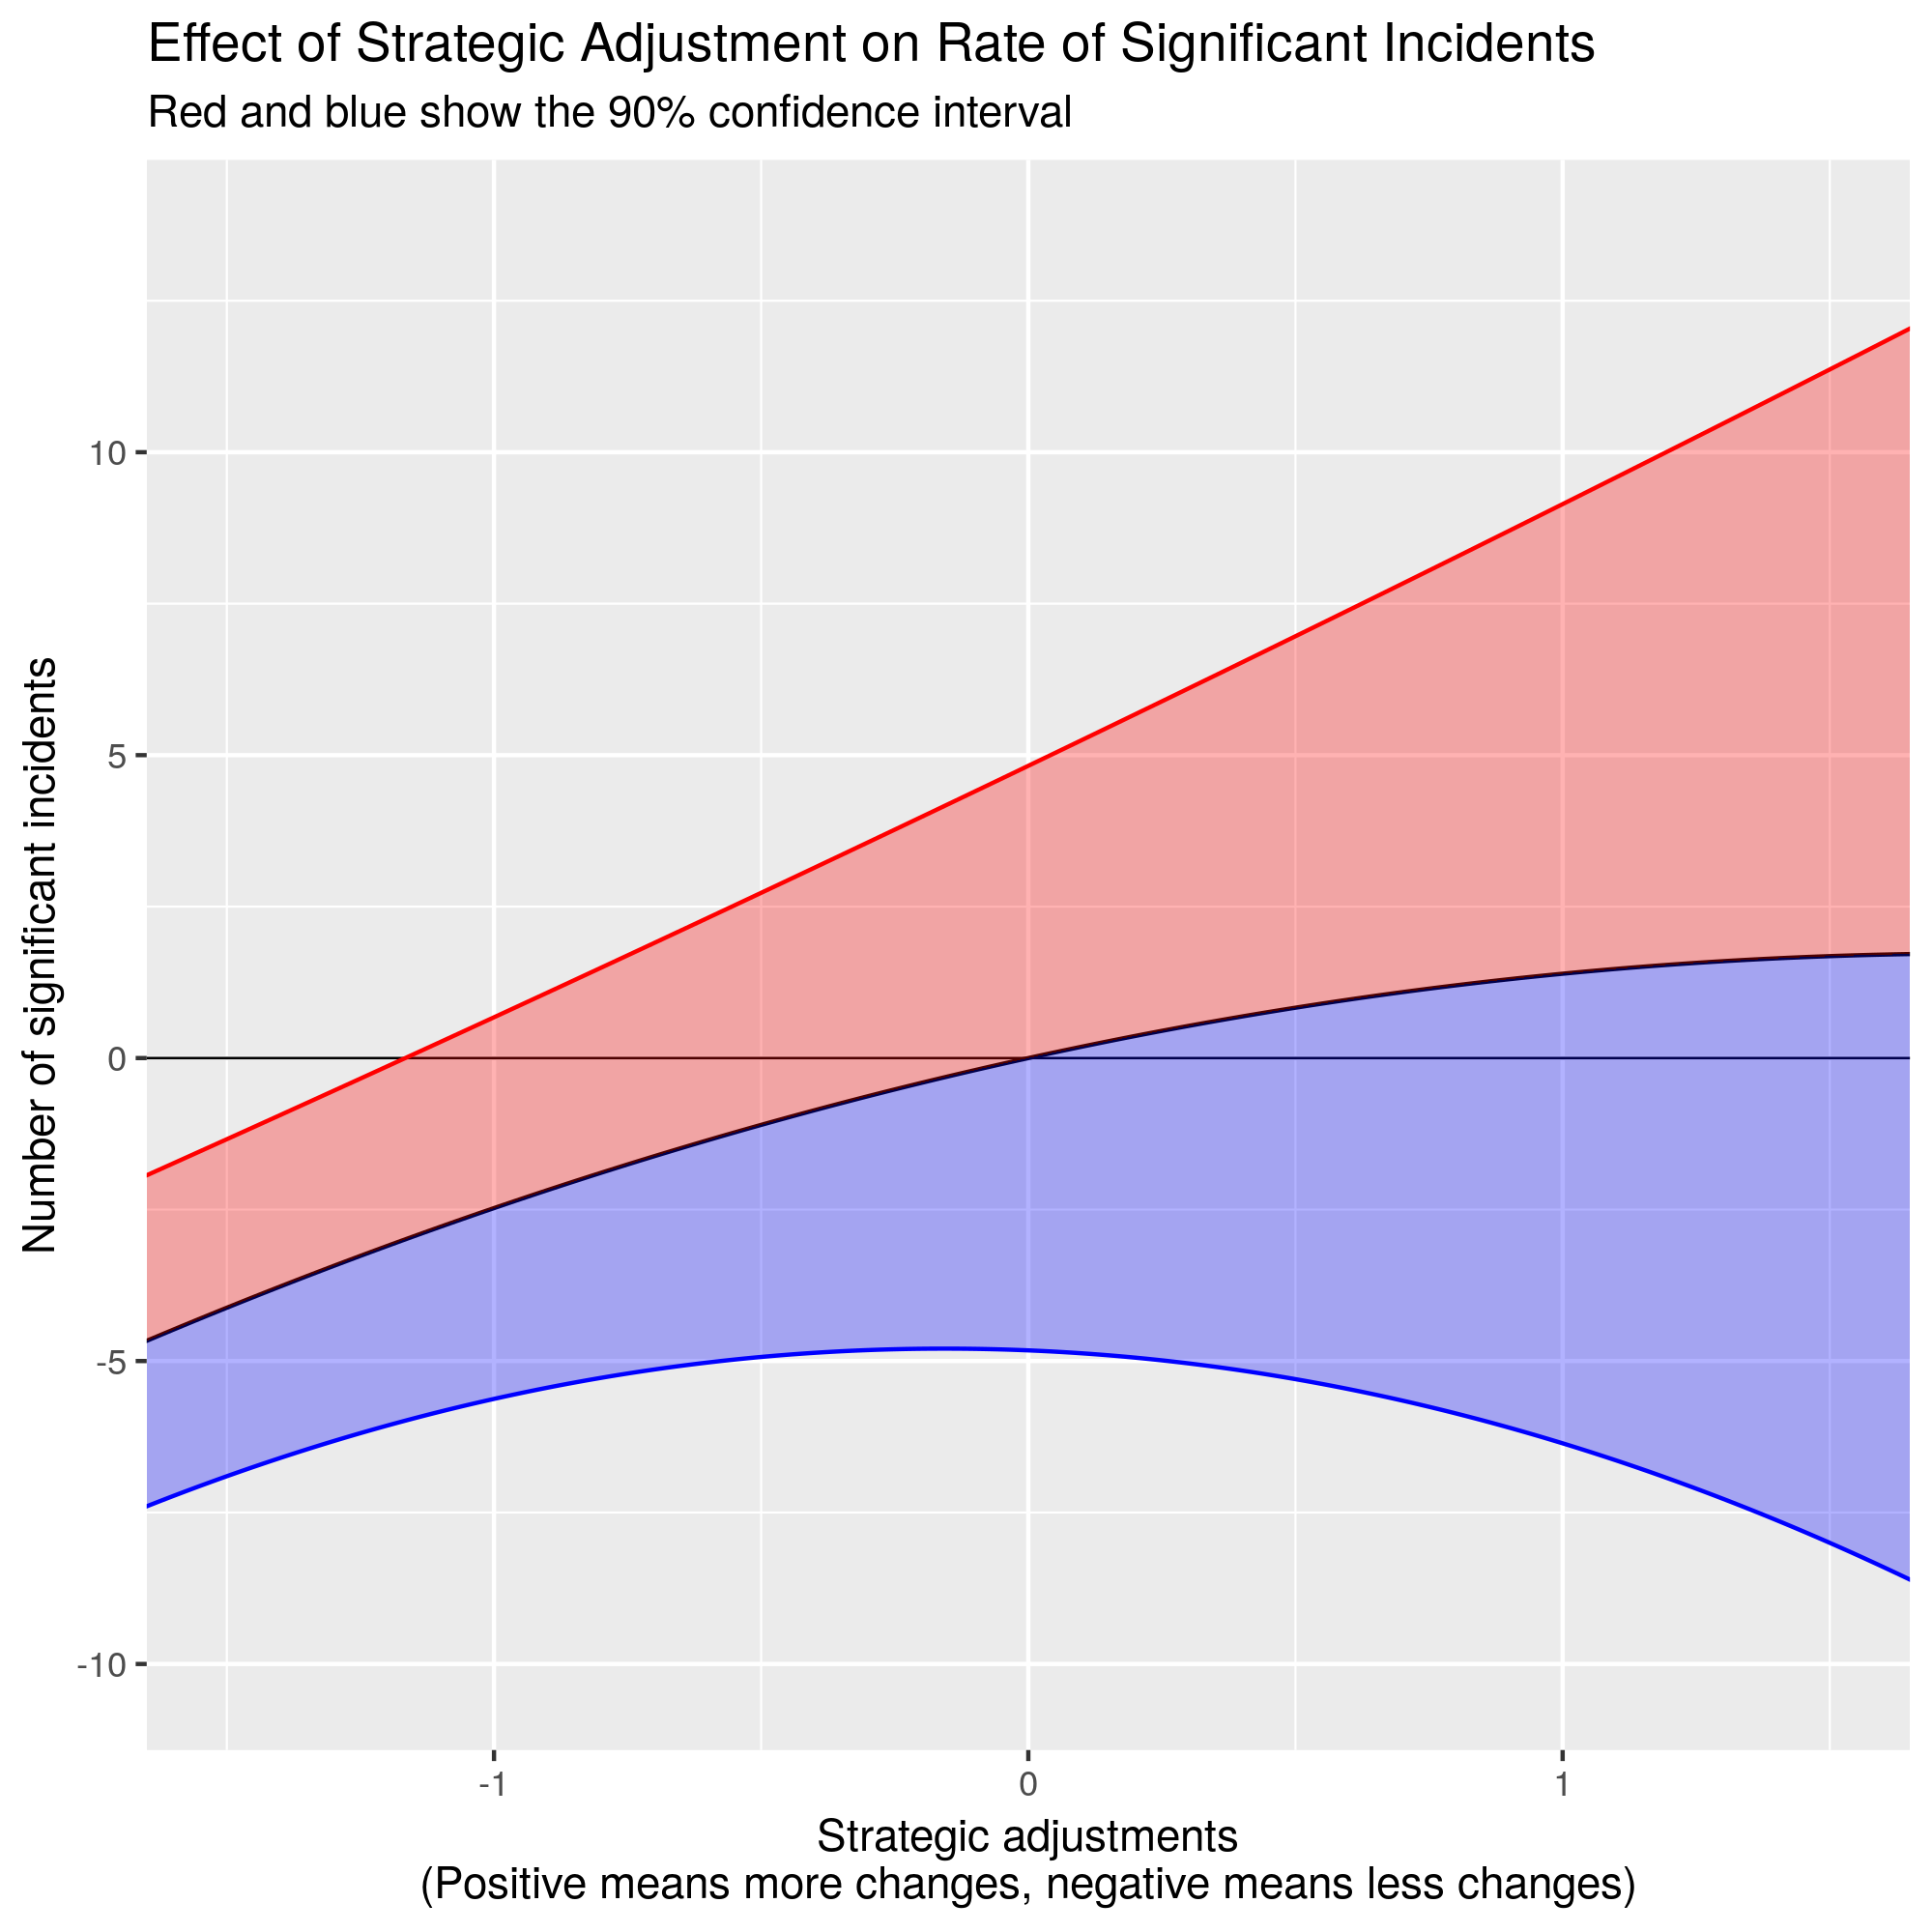
\includegraphics{illustrations/effect_size.png}
	\caption{}
\end{figure}


\section{Discussion and Conclusion}
Our results imply that phases of stability facilitate learning toward subordinate goals by suborganizations, whereas strategic adjustments might disrupt learning. \textit{Hypothesis 2} regarding the positive effect of stability is supported in four of the six models we ran, while there is only limited support for \textit{Hypothesis 1} regarding disruptions. The statistical model tests for within effects, and is more robust than a traditional GLS regression would be; there is also support in one of the two models that control for year effects. While the results are not yet fully persuasive, they do indicate that at least the research direction has merit. 

There is a large literature on how organizations can learn from one-off events, such as the Deepwater Horizon disaster \citep[e.g.,][]{March1991, Haunschild2015}. The context of pipeline incidents might provide more evidence of how organizations intentionally or unintentionally (at a macro level) steer the safety record of their organizations. One could assume that similar factors play a role in both the smaller accidents which we study in this paper (and which often go unreported in the media), and the larger accidents which affect large ecosystems (and occasionally threaten the survival of organizations): if this relationship between smaller and larger accidents exists, then the empirical context of this paper would be deserving of more attention indeed.

Two related levels of analysis exist that we have not touched on so far. One is the question of the positive impact of technology, and one is that of the potential impact of accidents on organizational environmental (and social) performance and organizational survival. We have controller for technology in our empirical analysis by including variable on the age of the pipeline network. In a context where the level of change in technology is considerable, the positive impact from technological modernization might by far outweigh any negative impacts from organizational processes.  When the impacts of an observation (accident) at the extreme end are considerable on the other hand (such as the impact of the Deepwater Horizon disaster on the Gulf of Mexico), the implications are the inverse of those of technology: these rare events then need to be taken into consideration when questions of environmental impacts and survival are discussed. Environmental performance is typically measured as the environmental footprint, or in a lifecycle analysis. To assess this impact, a consulting firm will look at regular inputs and outputs. Inputs can be decreased through simple efficiency-improving measures, such as the procurement of more energy-efficient equipment, or raw materials with a lower environmental impact. More and more we live in a world however that is shaped and threatened by rare events \citep{Beck1992}. If managerial actions have some impact on the occurrence of these rare events, then we should move these actions into sharper focus. Besides, managerial action that impacts likelihood of incidents could have also prevented the bankruptcy of the pipeline operator HVI Cat Canyon that was mentioned in the introduction.

The relationship of managerial steering and long-run impacts is already studied in the literature on temporality. That literature speaks to our context: organizational outcomes can be improved when firms plan ahead and create long-term roadmaps in addition to the short and mid-term business plans that companies necessarily have \citep{Slawinski2015}. On the other hand, a very short-sighted planning approach in conjunction with frequent directional changes will lead to inferior outcomes \citep{Bansal2014, Morales-Raya2015}.

Our paper still has some shortcomings that need to be addressed. Most importantly, our dataset so far mostly contains data from the FERC. Financial data on the organizations, such as expenditure and revenue of the organizations could be added; this would allow us to isolate the effects of interest better. In particular, companies that come under financial pressure might sacrifice pipeline safety in a (myopic) bid to improve the profit margin. Compustat and other databases provide data not only at the organization, but also at the business unit level (e.g., revenue of pipeline business as reported for that sector in the annual report); merging in that data would be particularly effective. There is also more data in the dataset itself that should be sighted: which are the organizations that make many adjustments, and why? Further, in the FERC data the incidents are described in enormous detail; \citet{Park2019} for example leverages this information better than we do at the moment. Finally, our analysis is backed by limited institutional knowledge. If we were to substitute the empirical analysis with e.g., interviews, we could gain more insights on other factors that affect incident rates, and the relationships at play. On a more practical note, considering that our sample size ranges from 401 to 624, and missingness (as well as our construction of variables as multi-year averages) reduces the effective observation period to 2004-2015 (with the effective years being listed in the fixed-effect regression as a result ranging from 2007-2012), we can also do more to leverage the statistical power of the available data. Finally, some operators have only very small pipeline networks; the range of their change variables (which is measured in percent) is therefore very large. The dataset could be tailored to limit the impact of this source of noise.

%\section{conclusion}
\bibliography{bibliography}
	
\end{document}